% =====================================================================
%  Mapping Natural-Disaster Damage from Satellite Imagery
%  Final report. Every number comes from results/ in the repository.
% =====================================================================
\documentclass[10pt,twocolumn]{article}

\usepackage[T1]{fontenc}
\usepackage[utf8]{inputenc}
\usepackage{lmodern}
\usepackage{microtype}
\usepackage[htt]{hyphenat}      % let \texttt identifiers hyphenate instead of
                                % stretching the line they sit on
\usepackage[a4paper,margin=1.9cm,columnsep=0.75cm]{geometry}
\usepackage{graphicx}
\usepackage{booktabs}
\usepackage{amsmath}
\usepackage{xcolor}
\usepackage{caption}
\usepackage{subcaption}
\usepackage{enumitem}
\usepackage{fancyhdr}
\usepackage[hidelinks]{hyperref}

% ---------------------------------------------------------------- style
\definecolor{accent}{HTML}{1F4E79}
\definecolor{accentbg}{HTML}{EAF0F7}
\definecolor{warnbg}{HTML}{FDF1E3}

\captionsetup{font=small,labelfont={bf,color=accent},skip=4pt}
\setlength{\parskip}{0pt}
\setlength{\emergencystretch}{3em}
\setlength{\tabcolsep}{4pt}     % default 6pt overflows the column in a 2-col layout
\tolerance=1200

\renewcommand{\topfraction}{0.92}
\renewcommand{\bottomfraction}{0.7}
\renewcommand{\textfraction}{0.07}
\renewcommand{\floatpagefraction}{0.75}
\setcounter{topnumber}{3}
\setcounter{totalnumber}{5}

\pagestyle{fancy}
\fancyhf{}
\renewcommand{\headrulewidth}{0.4pt}
\fancyhead[L]{\footnotesize\color{accent}Mapping Natural-Disaster Damage from Satellite Imagery}
\fancyhead[R]{\footnotesize\color{accent}\thepage}

\newcommand{\keybox}[2]{%
  \begin{center}
  \setlength{\fboxsep}{8pt}%
  \colorbox{#1}{\begin{minipage}{0.90\columnwidth}\small #2\end{minipage}}%
  \end{center}}

\newcommand{\wkeybox}[2]{%
  \begin{center}
  \setlength{\fboxsep}{8pt}%
  \colorbox{#1}{\begin{minipage}{0.965\textwidth}\small #2\end{minipage}}%
  \end{center}}

\newcommand{\class}[1]{\textsf{#1}}

% =====================================================================
\begin{document}

\twocolumn[
\begin{@twocolumnfalse}
\begin{center}

{\LARGE\bfseries Mapping Natural-Disaster Damage from Satellite Imagery\par}
\vspace{3pt}
{\large Cross-disaster transfer on xBD: pretrained versus from-scratch change-detection CNNs\par}

\vspace{8pt}
{\normalsize Artur Zavistovskyi, Bhuvanesh Dinesh Wadhwani, Anastasiia Khitrova, Yitian Zhou\par}
\vspace{2pt}
{\footnotesize Deep Learning Final Project\par}

\vspace{10pt}
\end{center}

\wkeybox{accentbg}{
\textbf{Abstract.} We assess per-building damage from paired pre- and post-disaster satellite imagery
on xBD, and measure whether a model trained on one family of disasters transfers to a family it has
never seen. Two siamese change-detection CNNs, one on an ImageNet-pretrained ResNet-18 encoder and
one on a compact encoder trained from scratch, are trained on 14 non-fire events using identical
patches, splits and class weights, then evaluated in-distribution and zero-shot on five wildfire
events held out entirely. In-distribution the pretrained model reaches \textbf{0.808 accuracy /
0.650 macro-F1}; on unseen wildfire it drops to \textbf{0.774 / 0.429}, a 33.9\% relative loss in
macro-F1. That headline is misleading: \class{destroyed} scores \emph{higher} out of domain than in
it (F1 0.758 versus 0.687), \class{no-damage} precision reaches 0.966, and threshold-free ROC-AUC
holds at 0.814. The collapse is confined to the two intermediate classes, 19.1\% of training patches
but only 1.7\% of wildfire patches, so the features transfer while the decision calibration does not.
Pretraining wins on every split and every metric, adding $+0.143$ accuracy and $+0.052$ macro-F1 on
wildfire. In Part 3, joining 185,045 labelled buildings to census block groups, an apparently
significant income gradient in damage ($\beta = +0.225$, $p = 0.0009$) disappears once event fixed
effects enter ($\beta = +0.057$, $p = 0.44$): who was hit is explained by \emph{which} disaster
struck, not by income within a disaster.
}
\vspace{9pt}
\end{@twocolumnfalse}
]

% =====================================================================
\section{Introduction}

Rapid damage maps are useful only if they can be produced \emph{before} labelled data for that
disaster exists. That makes the operational question sharper than ordinary image classification: not
``how accurate is the model'' but ``how accurate is it on a disaster type it has never seen''.

We study this on xBD~\cite{xbd}, the dataset behind the xView2 challenge~\cite{xview2}, which pairs
pre- and post-event high-resolution satellite tiles with building footprints and a four-level damage
scale. Prior work on this data fuses the two time steps inside the network~\cite{fusion}; we keep the
comparison explicit in the head instead, for the reason given in
Section~\ref{sec:arch}. The task is \emph{change detection at
building level}: given two co-registered crops of the same structure, one before and one after the
event, predict \class{no-damage}, \class{minor-damage}, \class{major-damage} or \class{destroyed}.

The experiment deliberately avoids a random split. Five wildfire events are removed from training
entirely and used as a zero-shot test set, while the official xView2 evaluation directories give an
in-distribution reference measured on the same trained model. The \emph{gap} between those two
numbers is the result; neither is informative alone.

\section{Data}

\subsection{Source and access}

We use the full xBD release: 11,034 scenes over 19 events, each contributing a $1024\times1024$ RGB
pre-disaster tile, the matching post-disaster tile, and a GeoJSON label file. That is 22,068 images
and \textbf{425,368} annotated building polygons on the post-disaster side, obtained through a
public mirror of the xView2 challenge release.\footnote{Kaggle dataset
\texttt{qianlanzz/\allowbreak xbd-dataset}, layout
\texttt{xbd/\{hold,\allowbreak test,\allowbreak tier1,\allowbreak tier3\}/\allowbreak \{images,\allowbreak labels\}}.}

Two properties were verified rather than assumed. \textbf{The tiles are already co-registered}:
pixel $(x,y)$ is the same ground location before and after, which is what makes cropping the
\emph{same} bounding box from both valid; without it the siamese design would compare different
places. And \textbf{the format is uniform}: all 800 files in a stratified quality-control sample
decode as $1024\times1024$ RGB PNG with no read errors, so no resolution standardisation or band
alignment is needed. Damage labels live only in the post-disaster GeoJSON, under
\texttt{features.xy[].\allowbreak properties.\allowbreak subtype}; the same file carries \texttt{features.\allowbreak lng\_lat}, giving
per-building WGS84 coordinates, so the geo-referencing for Part 3 is already present.

\subsection{Split design}

The split is scene-level and was produced by a dedicated indexing script rather than inside a
training notebook, so every model in the project trains on an identical partition
(Table~\ref{tab:splits}).

Two design points are worth defending. \texttt{test\_id} is drawn from the official \texttt{test} and
\texttt{hold} directories, which were never in any training pool and, unlike \texttt{val}, were never
used for tuning, which makes them an honest reference for the headline number. And assignment happens
at \emph{scene} level, which guarantees that the pre- and post-disaster image of a location cannot
separate and that no building can appear in two splits.

\begin{table}[t]
\centering
\footnotesize
\caption{Split design and sizes. Only \texttt{train}/\texttt{val} depend on the random seed; both
test sets are defined by the data itself.}
\label{tab:splits}
\begin{tabular}{@{}llrr@{}}
\toprule
\textbf{Split} & \textbf{Rule} & \textbf{Scenes} & \textbf{Polygons} \\
\midrule
\texttt{train}     & tier1+3, non-fire   & 3,135 & 225,506 \\
\texttt{val}       & tier1+3, non-fire   &   392 &  30,794 \\
\texttt{test\_id}  & test+hold, non-fire & 1,135 &  91,755 \\
\texttt{test\_ood} & wildfire, all       & 6,372 &  77,313 \\
\midrule
\multicolumn{2}{@{}l}{Total}             & 11,034 & 425,368 \\
\bottomrule
\end{tabular}
\end{table}

The five held-out events are \texttt{pinery-bushfire}, \texttt{portugal-\allowbreak wildfire},
\texttt{santa-\allowbreak rosa-wildfire}, \texttt{socal-fire} and \texttt{woolsey-fire}. An automated check
confirms zero wildfire scenes in \texttt{train} or \texttt{val}, and zero event overlap between the
training pool and \texttt{test\_ood}.

% =====================================================================
\section{Exploratory analysis}

\subsection{Class imbalance is severe and split-dependent}

\class{no-damage} accounts for 72.0\% of training polygons and the rarest class is $11.6\times$
smaller (Fig.~\ref{fig:classdist}). More importantly the composition is not stable across splits:
\texttt{test\_ood} is 80.2 / 0.9 / 0.9 / 14.7\% against 72.0 / 9.7 / 8.4 / 6.2\% in \texttt{train}.

Plain accuracy is therefore close to useless: always predicting \class{no-damage} scores 0.72 on the
training distribution while producing a damage map that never flags damage. We report macro-F1 and
per-class precision and recall as the decision metrics, use inverse-frequency class weights computed
on \texttt{train} only ($0.330 / 2.379 / 2.910 / 4.919$), and key checkpointing and early stopping on
validation macro-F1. Weighting was preferred to resampling: oversampling would repeat the same few
destroyed buildings many times per epoch and invite memorisation, while undersampling would discard
most of the majority signal.

\begin{figure*}[t]
\centering
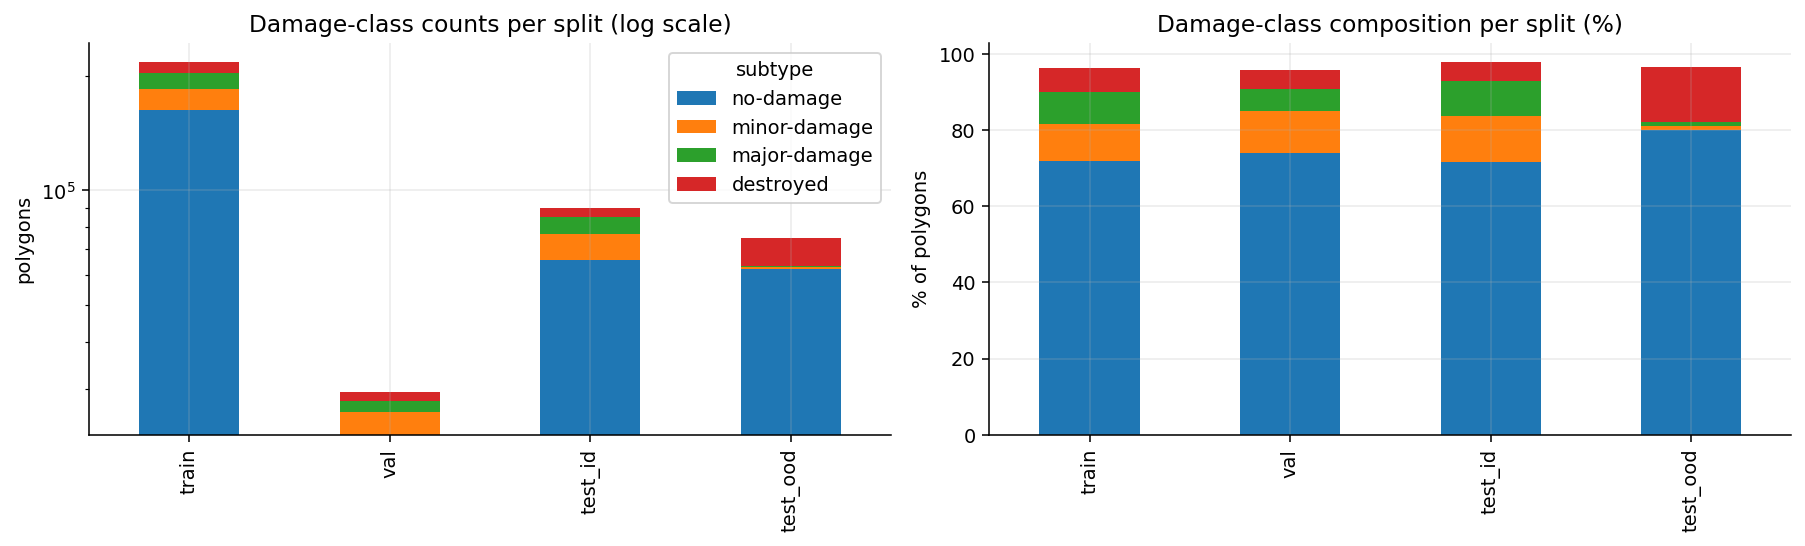
\includegraphics[width=0.85\textwidth]{figures/class_distribution_by_split.png}
\caption{Damage-class distribution per split. Left: counts on a log scale. Right: composition in per
cent. The \texttt{test\_ood} bar is qualitatively different from the other three, with the
intermediate classes almost vanishing and \class{destroyed} more than doubling.}
\label{fig:classdist}
\end{figure*}

\subsection{Wildfire damage is bimodal}

Averaged over events, the non-fire domain is 70.2 / 9.9 / 7.2 / 6.5\% across the four classes while
the wildfire domain is 78.8 / \textbf{1.2} / \textbf{1.1} / \textbf{14.8}\%. Fire either leaves a
building intact or destroys it; intermediate states barely occur. Figure~\ref{fig:heatmap} shows
this per event, and also how much the non-fire events differ among themselves:
\texttt{mexico-\allowbreak earthquake} is 99\% undamaged, \texttt{hurricane-\allowbreak matthew} is 51\%
\class{minor-damage}, \texttt{hurricane-\allowbreak harvey} is 35\% \class{major-damage}.

\begin{figure}[t]
\centering
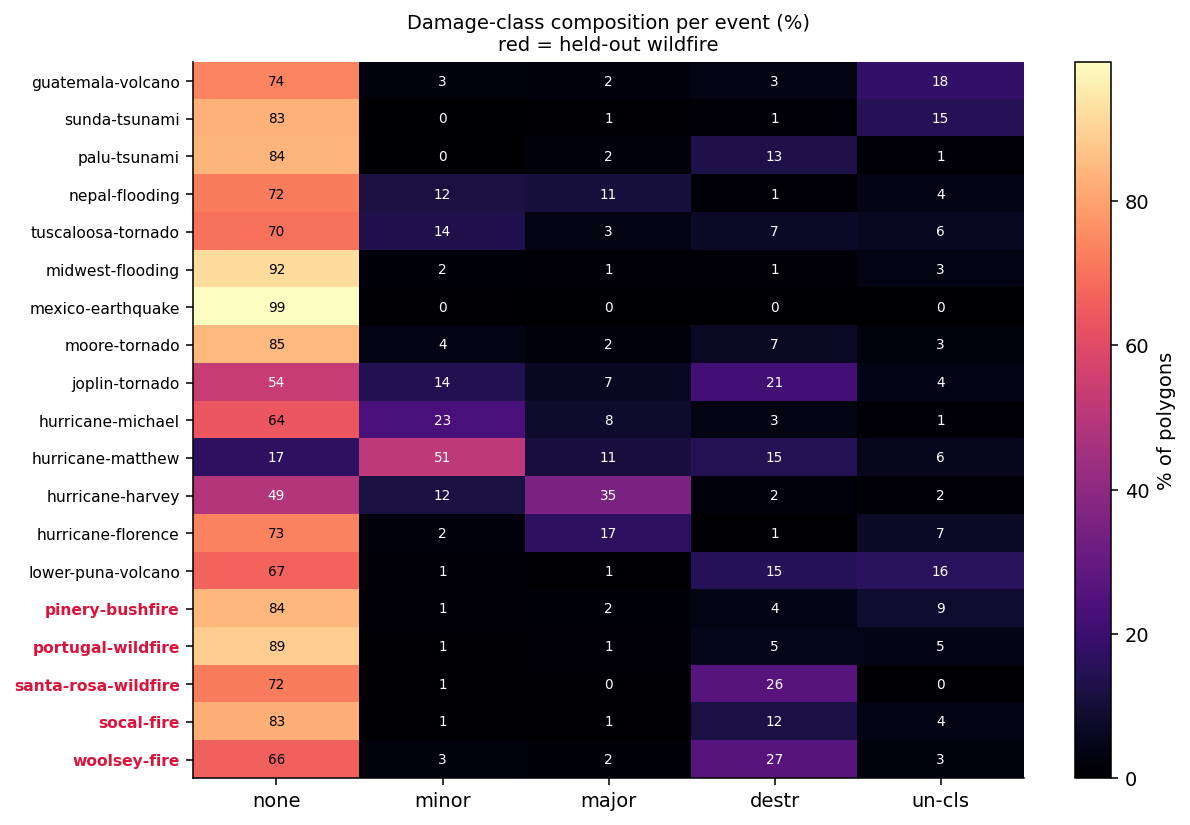
\includegraphics[width=\columnwidth]{figures/class_composition_by_event.png}
\caption{Damage-class composition per event, in per cent of that event's polygons. Held-out wildfire
events in red. The fire rows share a signature that no non-fire event reproduces: near-zero
\class{minor}/\class{major} with elevated \class{destroyed}.}
\label{fig:heatmap}
\end{figure}

This is the project's central hypothesis made measurable. A model that implicitly learns the
hurricane prior will be miscalibrated on fire \emph{even if its visual features transfer perfectly}.
It also says what to look for in the out-of-domain predictions: a pure prior shift produces errors
with a consistent direction, whereas failed features produce diffuse errors.

\subsection{Scene occupancy and patch size}

Empty scenes are common and strongly event-dependent (Fig.~\ref{fig:occupancy}): 9.8\% of training
scenes contain no buildings, against \textbf{54.1\%} of wildfire scenes, whose median building count
is zero, because the tier3 fire events cover large stretches of forest and scrubland. An empty scene
yields no samples but still costs a full $1024\times1024$ decode, so we sample only scenes with at
least five usable buildings. This is a \emph{sampling} decision, not a cleaning one: nothing is
deleted, and the identical rule applies to all four splits so it cannot tilt the comparison.

Buildings are small in absolute pixels: the median longest bounding-box side is 35 px and the 90th
percentile 64 px, with a thin tail to 349 px at the 99th. A $64\times64$ patch therefore covers
roughly 90\% of footprints at close to native resolution; larger mostly upsamples empty ground at
quadratic cost, smaller destroys the roof texture separating \class{minor} from \class{major} damage.
We keep a 10 px margin around each footprint, leaving a $44\times44$ px window for the building.
Damage is often more visible \emph{around} a building than on it (debris, scorch marks, standing
water), but the margin is kept modest deliberately, for reasons Section~\ref{sec:discussion} makes
concrete.

\begin{figure*}[t]
\centering
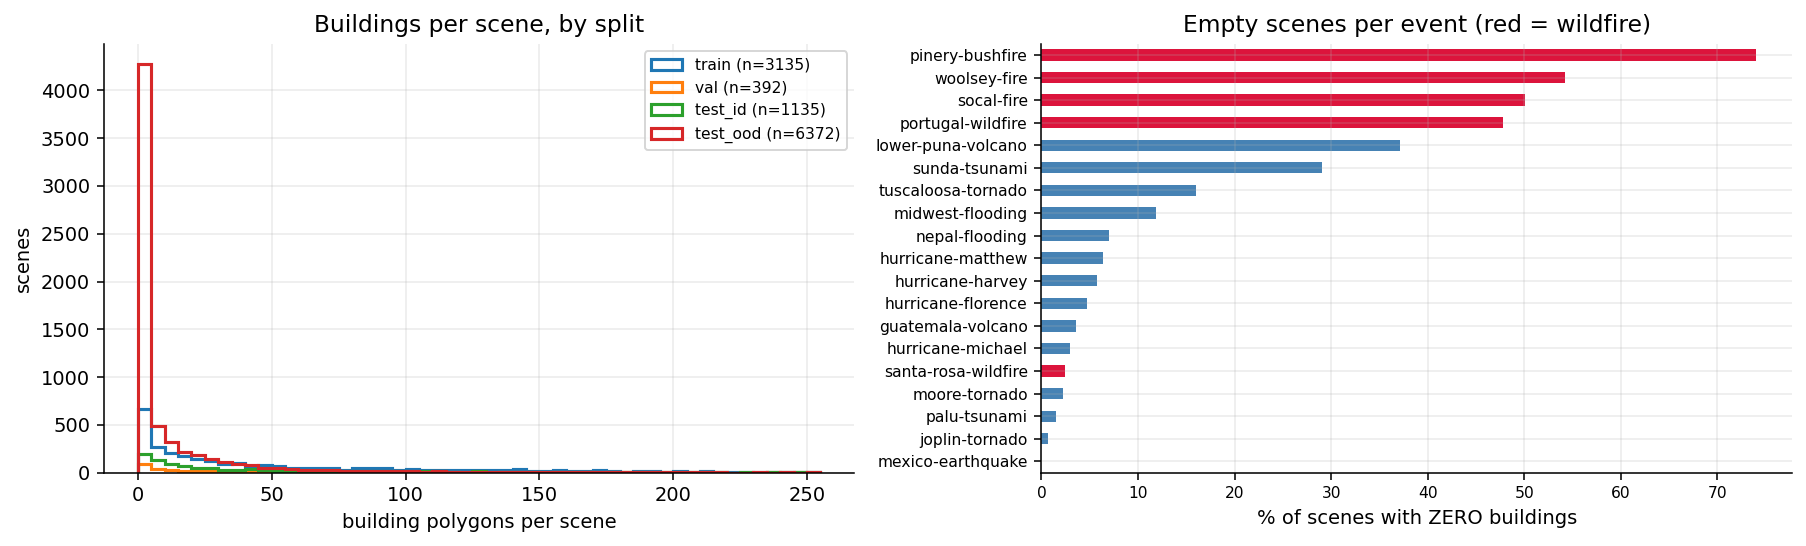
\includegraphics[width=0.85\textwidth]{figures/buildings_per_scene.png}
\caption{Left: distribution of building count per scene by split. Right: share of scenes with zero
buildings, per event (wildfire in red). Four of the five wildfire events are close to or above half
empty; pooled over all wildfire scenes the figure is 54.1\%.}
\label{fig:occupancy}
\end{figure*}

\subsection{A confound in the acquisition geometry}

Ground sample distance and off-nadir angle are similar across the two domains
($2.21 \pm 0.52$ against $2.12 \pm 0.31$ m, and $28.5 \pm 9.9$ against $25.6 \pm 6.0$ degrees), but
sun elevation is not: $64.4 \pm 7.5$ degrees for non-fire against $55.0 \pm 15.9$ for wildfire, with
a fire mode near $35^\circ$ that has no counterpart in training. Low sun means long shadows and a
materially different appearance for the same structure.

\keybox{warnbg}{\textbf{Honest caveat.} Those spreads are not what they look like, because every
scene within an event shares one acquisition. Statistically this is
\textbf{19 points, not 11,034}, and the geometry is
fully confounded with event identity: ``wildfire'' and ``the captures that happen to be wildfire''
cannot be separated on this data. Part of the transfer gap we report may be shadow length rather
than fire damage, and we cannot bound how much.}

\subsection{What the classes look like}

Figure~\ref{fig:examples} contrasts the two domains directly. In the non-fire domain the
post-disaster image usually retains the structure with altered geometry: torn roofs, debris,
standing water. Wildfire damage instead collapses a building to a uniform grey scar with the
footprint faintly visible, while \emph{undamaged} buildings often sit in surroundings that changed
completely (scorched vegetation) with the roof untouched.

That last observation generates a falsifiable prediction, made before any model was trained: a
change-detection model learns ``the scene changed'' $\Rightarrow$ ``the building is damaged'', so
under wildfire it should over-flag \class{no-damage}. Section~\ref{sec:results} reports the outcome.

\begin{figure*}[t]
\centering
\begin{subfigure}{0.46\textwidth}
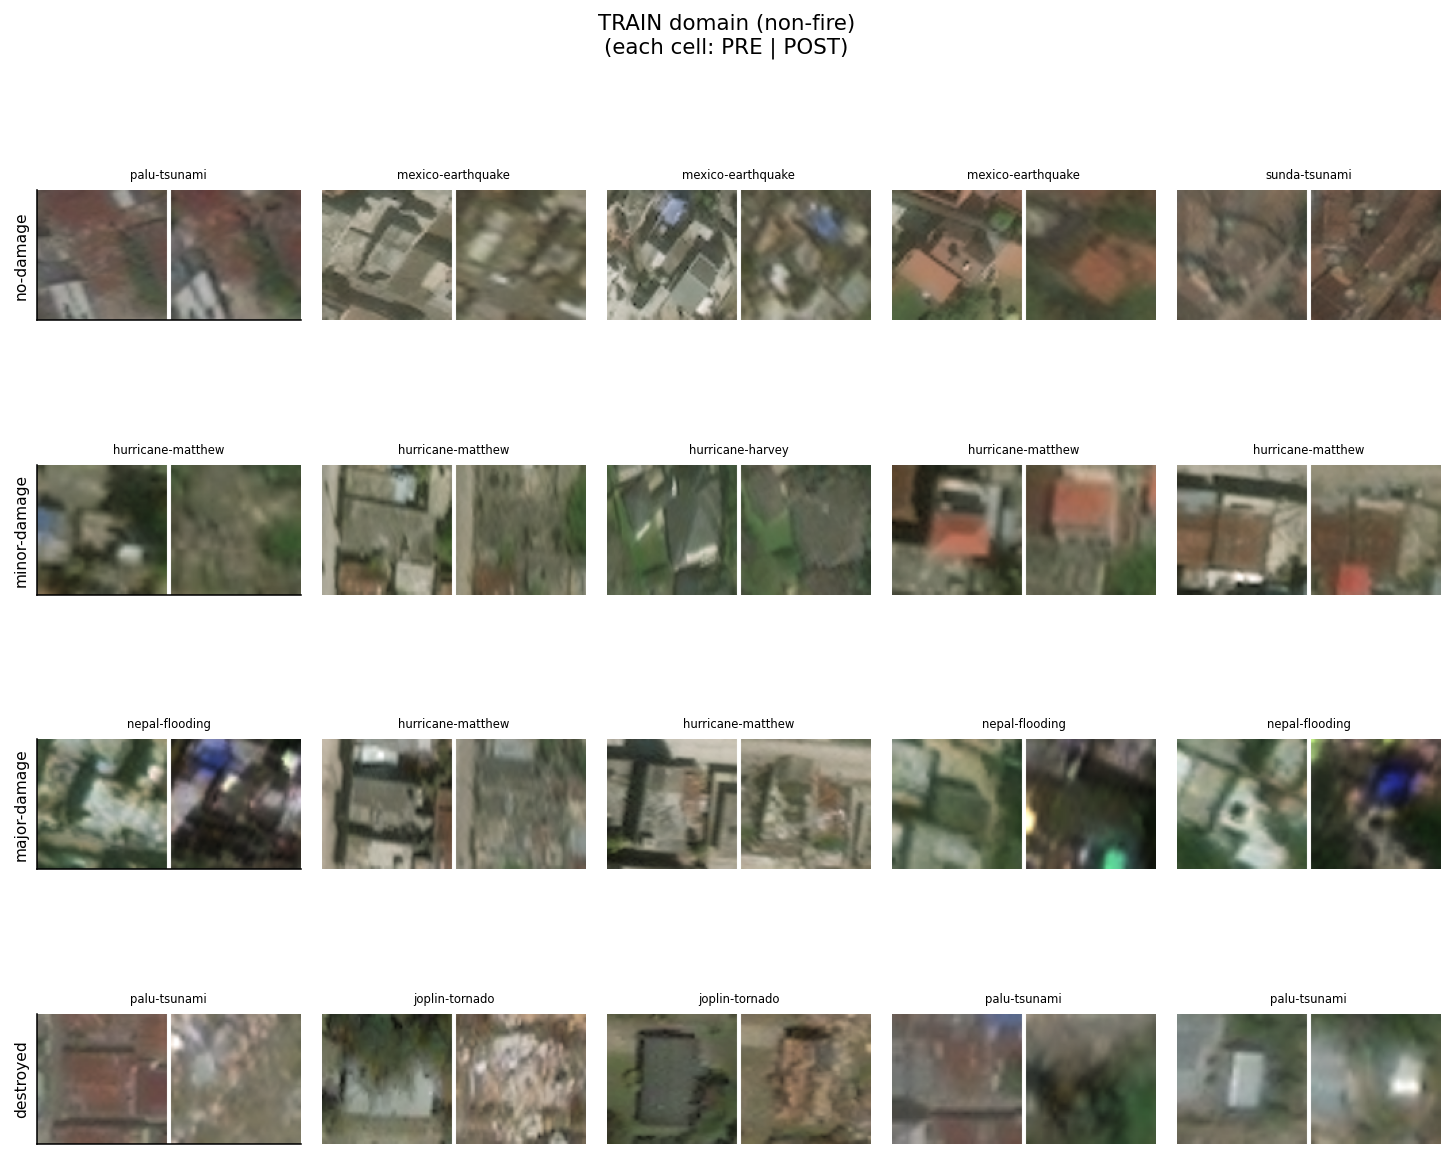
\includegraphics[width=\textwidth]{figures/examples_train.png}
\caption{Training domain (non-fire).}
\end{subfigure}\hfill
\begin{subfigure}{0.46\textwidth}
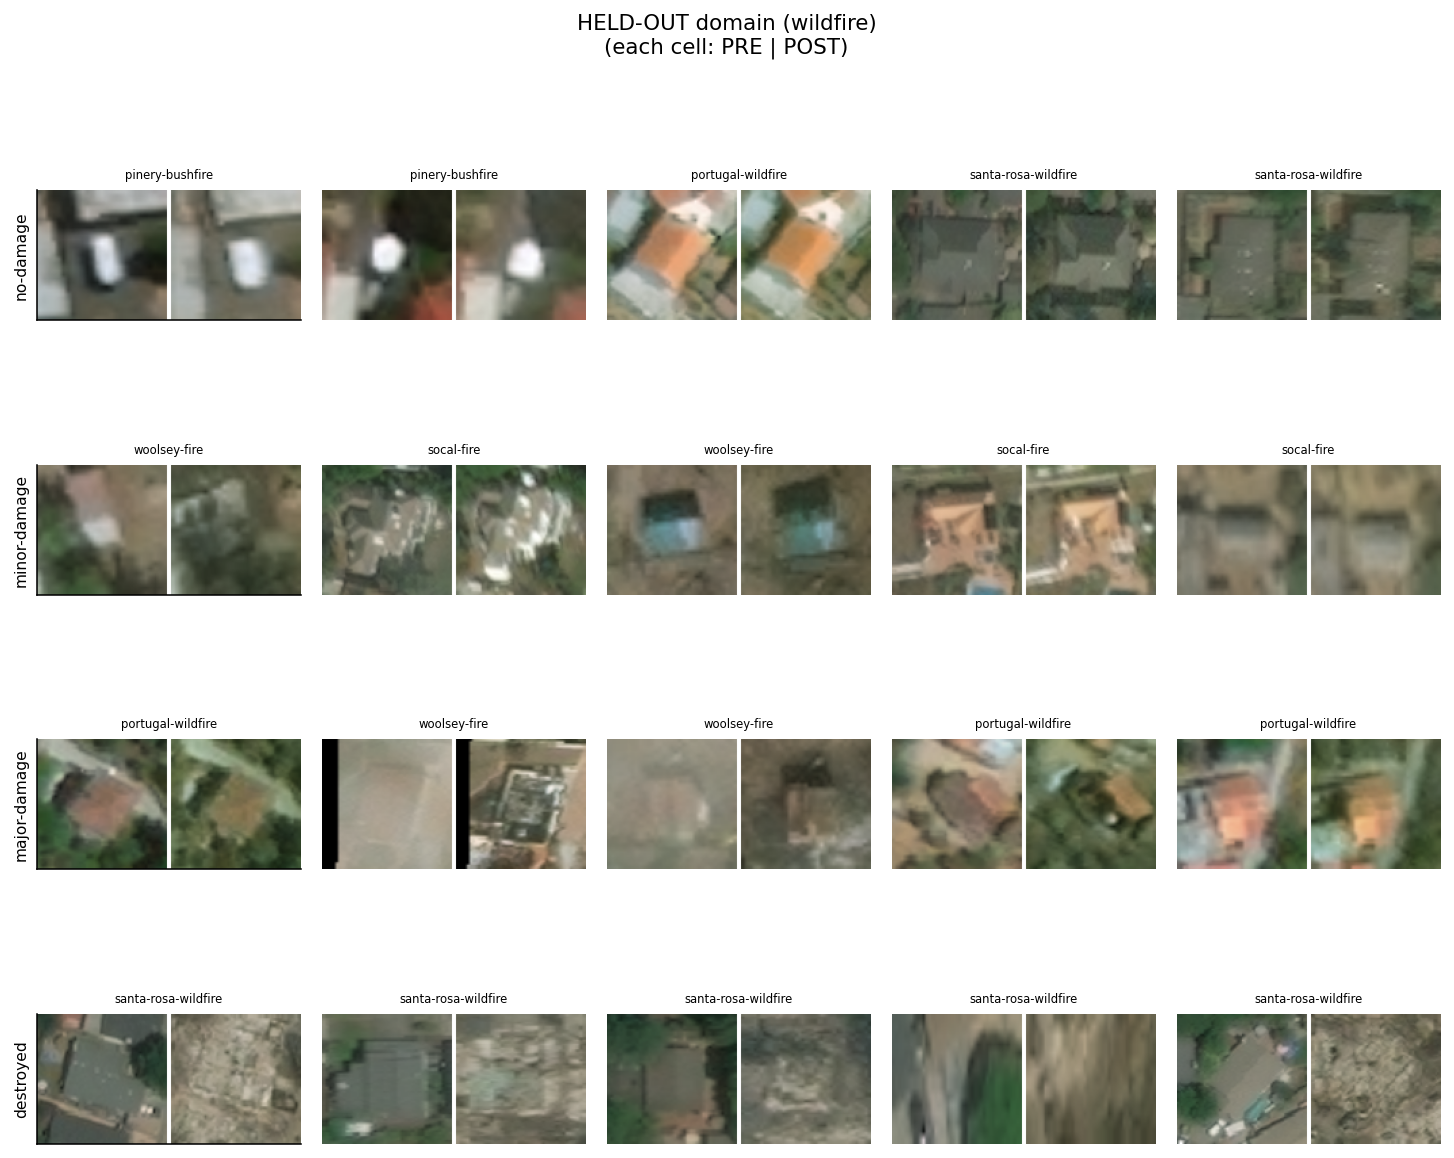
\includegraphics[width=\textwidth]{figures/examples_ood.png}
\caption{Held-out domain (wildfire).}
\end{subfigure}
\caption{Representative building patches, one row per damage class. Each cell shows the pre-disaster
crop on the left and the post-disaster crop on the right.}
\label{fig:examples}
\end{figure*}

% =====================================================================
\section{Data cleaning}

Nothing is removed silently. Every rule states its threshold, its cost and its per-split removal
rate, so a rule that quietly favours one split can be caught. Table~\ref{tab:cleaning} is the ledger.

\begin{table}[t]
\centering
\footnotesize
\caption{Cleaning ledger. Removal is reported against the scope each rule operates on. The 14
occlusion scenes and the 28 near-duplicate pairs were flagged for inspection, not deleted.}
\label{tab:cleaning}
\begin{tabular}{@{}llr@{}}
\toprule
\textbf{Rule} & \textbf{Scope} & \textbf{Removed} \\
\midrule
Missing / unpaired      & 11,034 scenes  & 0 \\
Corrupted images        & 800 files      & 0 \\
Unreadable labels       & 11,034 scenes  & 0 \\
Smoke / cloud           & 683 scenes     & 0 \\
\class{un-classified}   & 425,368 polys  & 14,011 \\
Degenerate polygons     & 425,368 polys  & 0 \\
Side $<8$ px            & 411,357 polys  & 14,458 \\
Near-duplicates         & 400 scenes     & 0 \\
\midrule
\multicolumn{2}{@{}l}{\textbf{Usable after cleaning}}    & \textbf{396,899} \\
\multicolumn{2}{@{}l}{\textbf{(93.3\% of 425,368)}}      & \\
\bottomrule
\end{tabular}
\end{table}

The two rules that cost data are the \class{un-classified} subtype (3.29\% of all polygons) and
sub-8-pixel footprints (3.51\% of the labelled remainder). Both were checked per split. The
\class{un-classified} rate is 3.67 / 4.08 / 2.09 / 3.30\% across
train / val / test\_id / test\_ood, and the tiny-footprint rate is 3.77 / 3.30 / 2.99 / 3.49\%.
Neither is concentrated in \texttt{test\_ood}, so neither flatters the transfer result.

\subsection{The occlusion question: a negative result}

The team's open data-quality question was whether images obscured by smoke should be removed.
\textbf{xBD carries no occlusion label}: the metadata block contains only capture geometry. The
closest available proxy is the \class{un-classified} subtype, which annotators used when a building
could not be assessed.

We ranked scenes by that proxy and tested it against four whole-tile statistics, chosen because
smoke and thin cloud on 3-band optical imagery are bright, low-contrast, low-saturation and
edge-poor. The sample is enriched deliberately, a 400-scene stratified quality-control sample plus
the 300 scenes with the highest \class{un-classified} rate, so the diagnostic has range on the proxy
rather than relying on chance coverage. Over the 505 tiles with a measurable rate the Spearman
correlations are $-0.366$ (edge density), $+0.116$ (brightness), $-0.095$ (saturation) and $-0.035$
(contrast). Edge density is the only one with any strength, explaining about 13\% of the rank
variance: real, but nowhere near a usable filter. Brightness, the statistic smoke should raise most,
is essentially uncorrelated. Neither signal can be trusted alone, and that absence of correlation is
itself the finding.

\keybox{accentbg}{
\textbf{Result, and why nothing was removed.} Flagging the top 2\% of a composite occlusion score
returns \textbf{14 scenes}: 13 \texttt{sunda-tsunami} and 1 \texttt{lower-\allowbreak puna-volcano}, that is
cloud over non-fire events, and \textbf{none is a wildfire scene}. By split they are 11
\texttt{train} and 3 \texttt{val}, with \textbf{zero} in either test set. We flagged them and removed
nothing: there is no ground truth to validate a threshold against, nothing flagged touches a reported
metric, and occlusion is part of the deployment problem anyway, since a system running on real
post-disaster imagery will meet cloud and smoke. The negative result that matters is that the team's
original worry, smoke over wildfire, is not what the diagnostic finds.}

\subsection{Leakage checks}

A perceptual-hash duplicate test over the 400-scene quality-control sample returned 28 near-duplicate
pairs, 19 crossing a split boundary. This was investigated rather than waved through: every
cross-split pair traces back to a handful of low-texture tiles colliding with several \emph{different
events on different continents}. One \texttt{portugal-\allowbreak wildfire} tile alone matches tiles from
\texttt{nepal-flooding}, \texttt{hurricane-\allowbreak harvey}, \texttt{sunda-tsunami}, \texttt{palu-tsunami} and
\texttt{moore-tornado} at once, and one tile each from the last three of those is pairwise identical
at Hamming distance 0. A single wildfire tile cannot be five unrelated disasters on other continents.
The cause is hash degeneracy: a 64-bit difference hash of a low-texture tile (open water, unbroken
forest, solid cloud) collapses toward a constant, so flat tiles collide regardless of content. We find
no evidence of leakage, consistent with the scene-level split design.

% =====================================================================
\section{Method}

\subsection{Patch construction}

One sample is two $64\times64\times3$ \texttt{uint8} patches cropped from the \emph{same} pixel
bounding box in the pre- and post-disaster tile, plus one integer label. Because the tiles are
already co-registered no warping is required; preprocessing is crop, resize, scale to $[0,1]$ and
ImageNet normalisation. Augmentation (flips, 90-degree rotations, brightness jitter) is applied
\emph{identically} to both images of a pair, since independent jitter per branch would manufacture a
difference where none exists, which is precisely the signal the model is meant to measure.

Scenes were sampled under a compute budget, stratified by event and restricted to scenes with at
least five usable buildings, yielding \textbf{135,262} patch pairs from 1,698 scenes
(Table~\ref{tab:patches}). Patches are written to memory-mapped arrays rather than individual image
files, which keeps the working set on disk and the loader fast.

\begin{table}[t]
\centering
\footnotesize
\caption{Extracted patch pairs per split and class. Note the support for \class{minor} and
\class{major} in \texttt{test\_ood}: every per-class number we report for those two classes rests on
these counts.}
\label{tab:patches}
\begin{tabular}{@{}lrrrrr@{}}
\toprule
& \class{none} & \class{minor} & \class{major} & \class{destr} & \textbf{total} \\
\midrule
\texttt{train}     & 55,284 & 7,661 & 6,265 & 3,706 & 72,916 \\
\texttt{val}       & 15,701 & 2,571 & 1,164 & 1,010 & 20,446 \\
\texttt{test\_id}  & 20,500 & 2,840 & 2,512 & 1,421 & 27,273 \\
\texttt{test\_ood} & 12,056 & \textbf{116} & \textbf{138} & 2,317 & 14,627 \\
\midrule
\textbf{Total}     & & & & & \textbf{135,262} \\
\bottomrule
\end{tabular}
\end{table}

\subsection{Architecture}
\label{sec:arch}

The task is a comparison, not the classification of a single image. Using only the post-disaster
patch discards the reference, while stacking pre and post into a six-channel input forces the first
convolution to be relearned, throwing away the pretrained weights exactly where they transfer best.
Both models therefore use a \textbf{siamese encoder with shared weights} and a small head reading
\[
\big[\;f_{\text{pre}},\;\; f_{\text{post}},\;\; \lvert f_{\text{pre}} - f_{\text{post}}\rvert\;\big].
\]
The absolute difference is the explicit change signal; keeping the raw features alongside it lets the
head use appearance as well. Shared weights halve the parameter count and force both branches into a
common feature space, which is what makes the difference term meaningful.

\textbf{Model A (pretrained)} uses an ImageNet-pretrained ResNet-18~\cite{resnet,imagenet} encoder,
11.57M parameters in total. At a $64\times64$ input, depth stops paying: architectures designed for
224 px inputs downsample away the little spatial resolution available, and a vision transformer would
reduce a 64 px image to a handful of tokens without the data to compensate for the missing
convolutional prior. ResNet-18 also keeps the comparison honest, since a much larger backbone would
make any win attributable to size rather than pretraining.

\textbf{Model B (from scratch)} replaces that encoder with a compact stack built for this problem:
four blocks of two $3\times3$ convolutions with BatchNorm and ReLU followed by $2\times2$
max-pooling, at channel widths $32 \to 64 \to 128 \to 256$, then global average pooling. Total 1.37M
parameters. Everything downstream of the encoder is identical.

\subsection{Training}

Model A follows a linear-probe-then-fine-tune schedule~\cite{lpft}: phase 1 trains only the head on a
frozen backbone for 5 epochs at $10^{-3}$, so the randomly initialised head does not push large
gradients into good weights; phase 2 unfreezes \texttt{layer3} and \texttt{layer4} for up to 45
further epochs at $10^{-4}$, since early layers transfer essentially unchanged while the late
semantic layers must be repurposed. Model B has no pretrained weights to protect, so the whole
network trains from step one at $10^{-3}$ over the same 50-epoch budget.

Both use AdamW with cosine annealing, weight decay $10^{-4}$, weighted cross-entropy with the class
weights above, batch size 128, mixed precision, seed 42, early stopping on validation macro-F1 with
patience 8, and checkpointing on the same criterion. Both are implemented in
PyTorch~\cite{pytorch} and ran locally on an NVIDIA RTX 4070
Laptop GPU; Model A stopped after 43 epochs with the best checkpoint at epoch 35; Model B stopped
after 16 epochs with the best checkpoint at epoch 8, in 14.2 minutes at 53 s per epoch.

\begin{figure}[t]
\centering
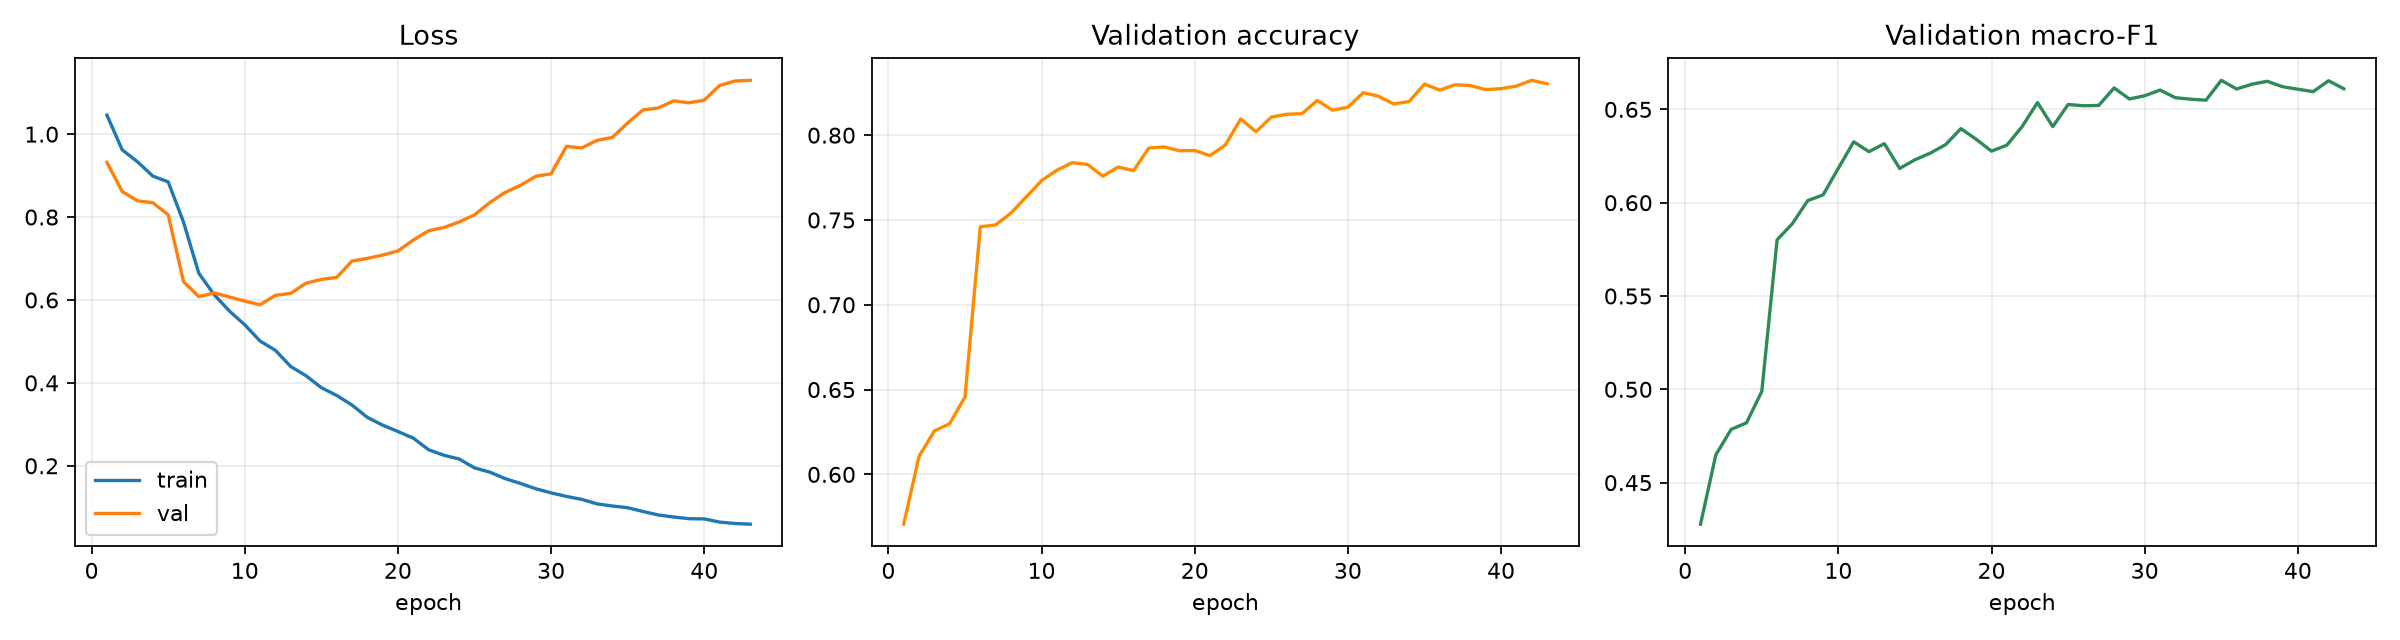
\includegraphics[width=\columnwidth]{figures/training_curves_pretrained.png}
\caption{Model A training history. Validation loss bottoms out at epoch 11 and then rises steadily,
while validation macro-F1 keeps improving to epoch 35. Model B shows the same pattern.}
\label{fig:curves}
\end{figure}

Two observations from the curves (Fig.~\ref{fig:curves}) are worth recording. Unfreezing lifted Model
A's validation macro-F1 from 0.499 to \textbf{0.580 in a single epoch}, the clearest evidence here
that a frozen ImageNet backbone is not sufficient for satellite imagery. And from its epoch-11
minimum (0.588) Model A's validation \emph{loss} climbs to 1.027 by the best checkpoint and 1.130 by
the end, while macro-F1 improves over the same stretch (0.633 to 0.666). Under a weighted loss on
imbalanced data this is expected, since the model grows over-confident faster than it grows wrong,
and it is why loss would have been the wrong early-stopping criterion. The same decoupling appears in
Model B, on a differently initialised network with a different schedule, so it is a property of the
objective rather than of one run.

% =====================================================================
\section{Results}
\label{sec:results}

\begin{table}[t]
\centering
\footnotesize
\caption{Headline results. Two trained models, three evaluation sets each. P is the pretrained
ResNet-18 encoder, S the from-scratch encoder. \texttt{val} and \texttt{test\_id} are seen disaster
types, \texttt{test\_ood} is the held-out wildfire set; the drops are \texttt{test\_id} to
\texttt{test\_ood}.}
\label{tab:main}
\begin{tabular}{@{}llrrr@{}}
\toprule
\textbf{Split} & & \textbf{Acc.} & \textbf{Macro-F1} & \textbf{AUC} \\
\midrule
\texttt{val}       & P & \textbf{0.830} & \textbf{0.666} & \textbf{0.910} \\
                   & S & 0.763 & 0.597 & 0.902 \\
\texttt{test\_id}  & P & \textbf{0.808} & \textbf{0.650} & \textbf{0.908} \\
                   & S & 0.768 & 0.615 & 0.903 \\
\texttt{test\_ood} & P & \textbf{0.774} & \textbf{0.429} & \textbf{0.814} \\
                   & S & 0.630 & 0.377 & 0.790 \\
\midrule
Abs. drop          & P & $-0.034$  & $-0.221$  & $-0.094$ \\
                   & S & $-0.138$  & $-0.238$  & $-0.113$ \\
Rel. drop          & P & $-4.2\%$  & $-33.9\%$ & $-10.4\%$ \\
                   & S & $-17.9\%$ & $-38.7\%$ & $-12.5\%$ \\
\bottomrule
\end{tabular}
\end{table}

Table~\ref{tab:main} gives the headline numbers. For both models \texttt{val} and \texttt{test\_id}
agree closely (0.666 against 0.650 macro-F1 for P, 0.597 against 0.615 for S), which matters: it
shows the in-distribution figure is not a lucky validation draw, so the \texttt{test\_ood} gap is a
genuine domain effect rather than noise.

\subsection{Per-class behaviour}

The aggregate drop is misleading, and the per-class view (Fig.~\ref{fig:perclass}) shows why.

\begin{figure*}[t]
\centering
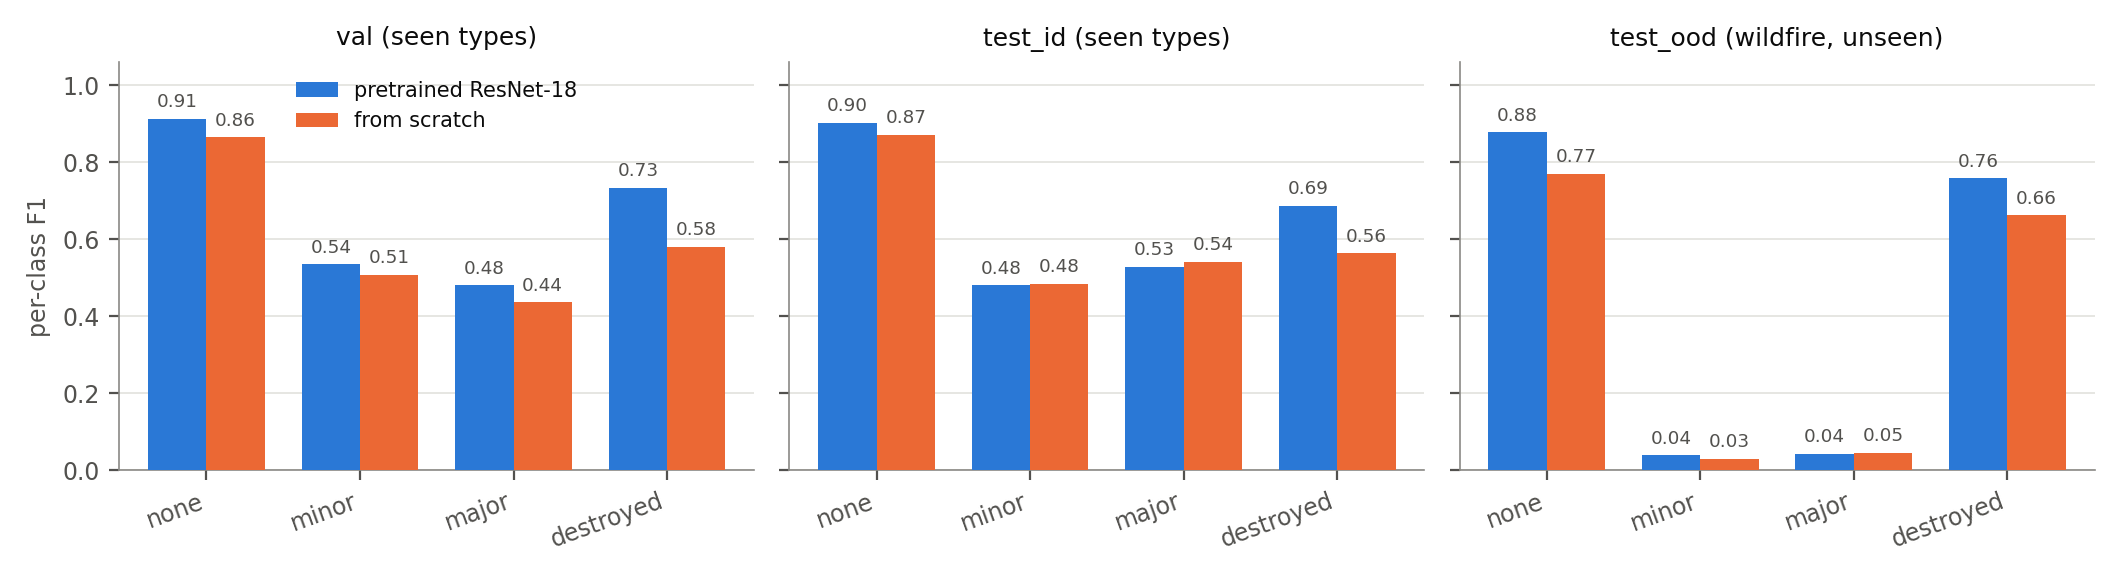
\includegraphics[width=0.85\textwidth]{figures/per_class_f1.png}
\caption{Per-class F1 for both models on the three evaluation sets. In domain the two are close on
the intermediate classes and pretraining mostly buys \class{destroyed}; out of domain both collapse
on \class{minor} and \class{major}, and the pretrained advantage on \class{destroyed} widens.}
\label{fig:perclass}
\end{figure*}

For the pretrained model, \class{destroyed} scores F1 0.758 on wildfire against 0.687 in domain, at
precision 0.872, and \class{no-damage} reaches precision 0.966. A model that has never seen a fire
recognises burnt-out buildings \emph{better} than it recognises hurricane destruction. The collapse
is confined entirely to the two intermediate classes, which fall from F1 0.480 and 0.529 in domain to
0.038 and 0.043 on wildfire. What breaks is precision, down to 0.020 and 0.024; their recall does not
vanish at all (0.284 and 0.203).

\subsection{Error structure}

Figure~\ref{fig:prior} makes the mechanism explicit by comparing the predicted class distribution on
\texttt{test\_ood} with the true one. Against 116 true \class{minor} and 138 true \class{major}
patches, the pretrained model emits 2,814 intermediate predictions and the from-scratch model 4,713,
an over-prediction of $11.1\times$ and $18.6\times$. That alone caps combined precision near 0.02
regardless of how good the features are.

\begin{figure}[t]
\centering
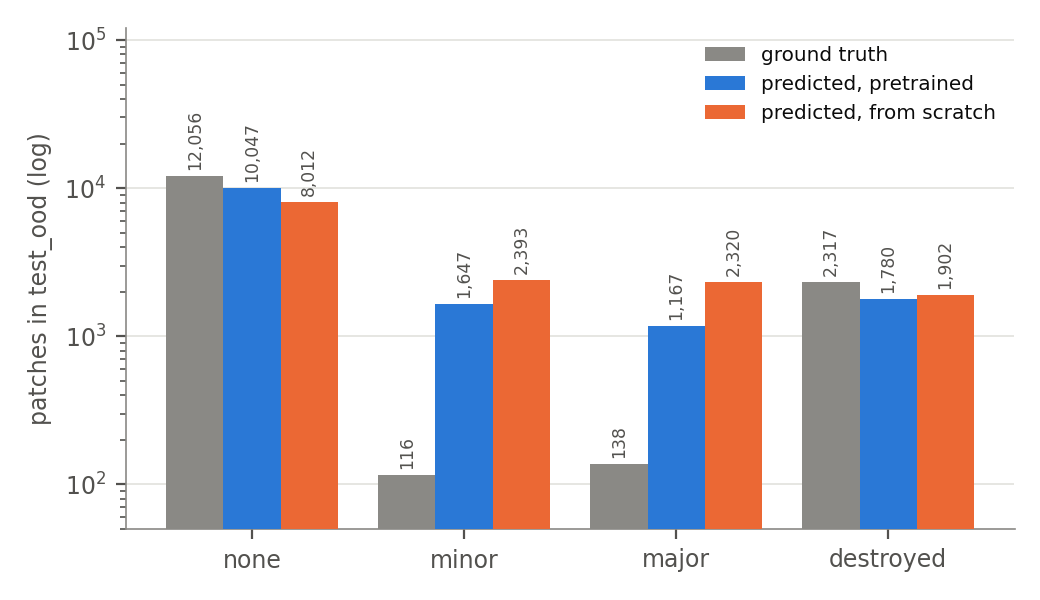
\includegraphics[width=\columnwidth]{figures/ood_prior_shift.png}
\caption{True against predicted class distribution on \texttt{test\_ood} (log scale). Both models
reproduce the shape of the training prior rather than the wildfire prior, heavily over-predicting the
two intermediate classes.}
\label{fig:prior}
\end{figure}

The direction of the errors is equally consistent. For the from-scratch model, whose full confusion
matrices are available (Fig.~\ref{fig:confusion}), \textbf{81.1\% of out-of-domain errors
over-estimate severity} against 18.9\% that under-estimate, and 35.9\% of truly undamaged wildfire
buildings (4,324 of 12,056) are flagged as damaged. The pretrained model shows the same failure mode
less severely: its \class{no-damage} recall of 0.805 on \texttt{test\_ood} corresponds to a
\textbf{19.5\% false-alarm rate}. Both confirm the prediction made from the exploratory analysis
before training.

\begin{figure*}[t]
\centering
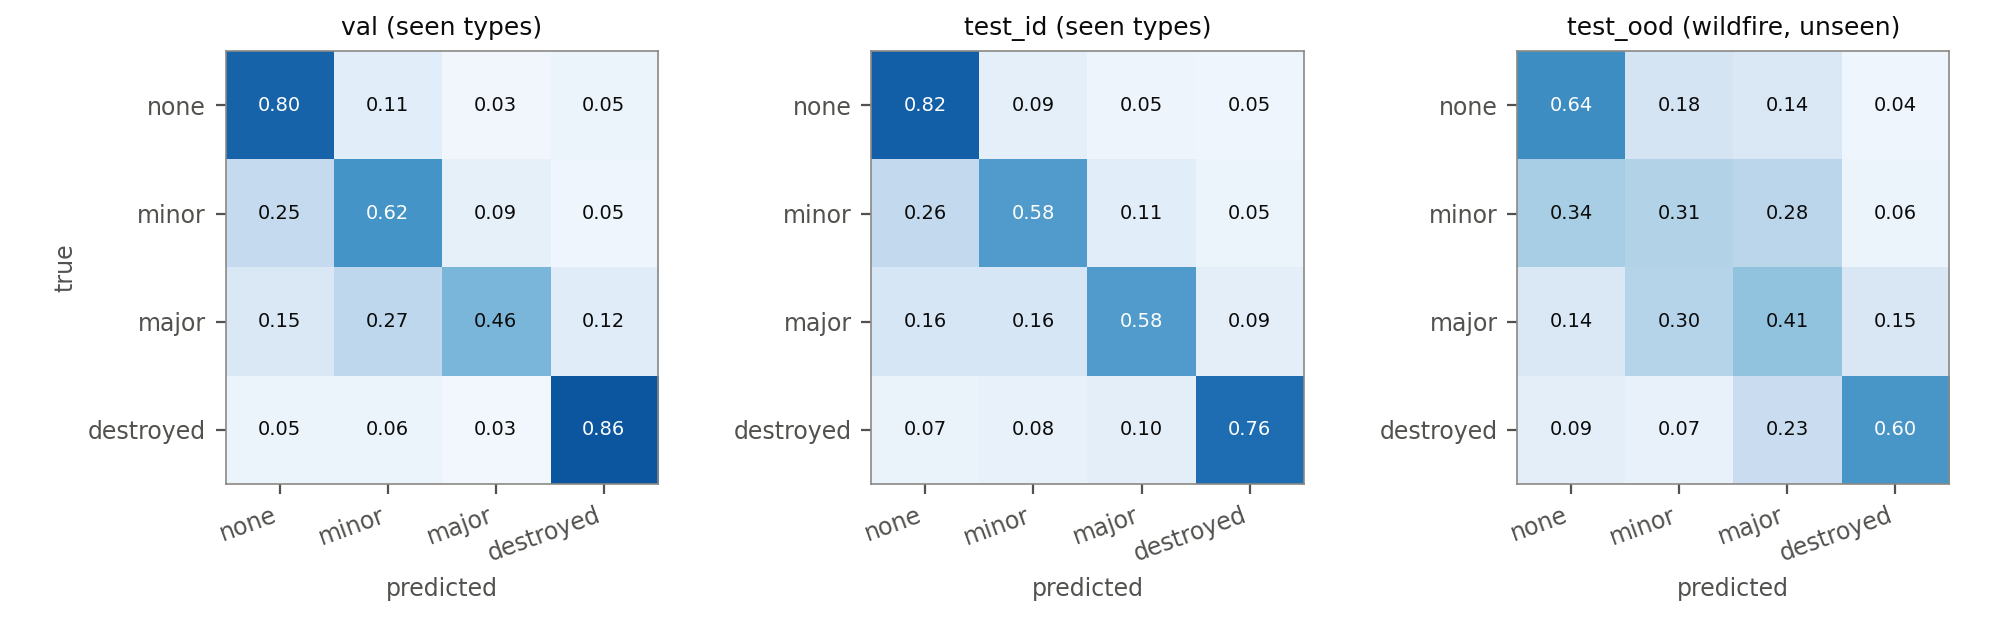
\includegraphics[width=0.85\textwidth]{figures/confusion_scratch.png}
\caption{Confusion matrices for the from-scratch model, normalised per true class (recall). The
\texttt{test\_ood} panel shows probability mass pushed off the diagonal in one direction, toward
greater severity, rather than scattered.}
\label{fig:confusion}
\end{figure*}

\subsection{Pretrained against from-scratch}
\label{sec:comparison}

Both models train on identical patches, splits, class weights and evaluation code, and differ only
in the encoder. Pretraining wins on every split and every metric in Table~\ref{tab:main}, and its
advantage is largest where it matters most: on \texttt{test\_ood} it adds $+0.143$ accuracy,
$+0.052$ macro-F1 (a 13.9\% relative gain over the from-scratch model's 0.377) and $+0.024$ ROC-AUC.
The relative macro-F1 drop from \texttt{test\_id} also shrinks, 33.9\% against 38.7\%, so pretraining
does not just raise the floor, it makes the domain-shift degradation proportionally smaller.

Per class, the clearest single difference is \class{destroyed}: 0.758 against 0.662 out of domain,
and 0.687 against 0.563 in it. The intermediate classes are indistinguishable between models because
both are far below usable precision, and at $n = 116$ and $n = 138$ the small reversals there are
within noise. One caveat: this is the assignment's required two-model comparison, but not a pure
pretraining ablation, since the pretrained encoder is also $8.4\times$ larger. A third run using the
same ResNet-18 with random initialisation would separate the two effects, and we have not run it.

% =====================================================================
\section{Discussion}
\label{sec:discussion}

\keybox{accentbg}{
\textbf{The features transfer; the calibration does not.} Four independent measurements support this
reading of the 33.9\% macro-F1 drop.
\emph{(1)} \class{destroyed} scores higher out of domain than in it (0.758 against 0.687) and
\class{no-damage} precision is 0.966: the two classes that actually occur under wildfire are
recognised well.
\emph{(2)} The errors move in one direction, 81.1\% over-estimating severity for the model where the
full matrix is available. A consistent bias is the signature of a shifted prior; failed
representations would produce diffuse, symmetric confusion.
\emph{(3)} ROC-AUC, which does not depend on a decision threshold, holds at 0.814 against 0.908 in
domain. The ranking survives; the boundary is what breaks.
\emph{(4)} The collapse is arithmetically forced. \class{minor} and \class{major} are 10.5\% and
8.6\% of training patches but 0.79\% and 0.94\% of wildfire patches. The pretrained model emits 2,814
intermediate predictions against 254 true cases, capping combined precision near 0.02 regardless of
feature quality, and matching the 0.020 and 0.024 actually measured.}

The distinction is not academic. A representation failure would mean the approach cannot be deployed
on a new disaster type at all. A calibration failure means the ranking is usable and only the
decision rule needs adjusting, a far more tractable problem with an established remedy in prior
correction~\cite{saerens}, which rescales class posteriors by the ratio of target to source priors
without retraining. Operationally, such a model deployed on an unlabelled new disaster type would
reliably separate destroyed from intact structures while badly over-reporting intermediate damage.
For triage, meaning ``where should responders look first'', that failure mode is comparatively
benign; for damage \emph{quantification}, and certainly for aid allocation, it is not.

% =====================================================================
\section{Impact and recovery analysis}
\label{sec:socio}

\subsection{Data and method}

To ask whether damage falls unequally across communities, we take the per-building WGS84 centroids in
the xBD labels, restrict to the ten US events for which census geography is available, and spatially
join them to 2020 TIGER census block groups. Each building contributes an ordinal damage score
(\class{no-damage} $= 0$ to \class{destroyed} $= 3$); the unit of analysis is the block-group mean.
Block groups with fewer than 20 buildings are dropped. That gives \textbf{185,045 buildings} in
\textbf{308} block groups, joined to American Community Survey covariates for 2017~\cite{acs}.

Two data-quality problems had to be handled first, and both are reported rather than absorbed
silently. \textbf{Census sentinel values}: the ACS extract encodes missing values as $-666666666$
rather than as nulls, and 17 of the 308 block groups carry one in median income, home value or year
built, which if left in place makes those coefficients meaningless. We drop them, leaving
\textbf{291} block groups. \textbf{Two unusable columns}: the poverty rate is empty for every block
group, and the hazard exposure proxy is identically zero because no fire-perimeter, storm-track or
coastline layer was ever joined. Both are dropped rather than reported as null effects.

The exposure control is therefore the built environment only (building density and median building
age), plus, in the strongest specification, \textbf{event fixed effects}. Event identity is the
sharpest exposure control this data supports: comparing two block groups inside the same disaster
holds the hazard roughly constant.

\subsection{Results}

\begin{table}[t]
\centering
\footnotesize
\caption{Standardised OLS coefficients on block-group mean damage score, $n = 291$. Each column adds
controls to the one before it: socioeconomic only, plus built environment, plus event fixed effects.}
\label{tab:socio}
\begin{tabular}{@{}lrrr@{}}
\toprule
& \textbf{naive} & \textbf{+ built} & \textbf{+ FE} \\
\midrule
Median income      & $+0.211^{**}$ & $+0.225^{***}$ & $+0.057$ \\
Median home value  & $-0.150^{**}$ & $-0.139^{*}$   & $-0.039$ \\
Renter share       & $+0.015$      & $+0.032$       & $-0.016$ \\
Building density   &               & $-0.085^{*}$   & $-0.103^{**}$ \\
Building age       &               & $-0.102^{*}$   & $-0.096^{*}$ \\
\midrule
$R^2$              & 0.045 & 0.072 & 0.225 \\
adjusted $R^2$     & 0.035 & 0.055 & 0.186 \\
\bottomrule
\end{tabular}
\vspace{2pt}
{\scriptsize $^{*}p<0.05$, $^{**}p<0.01$, $^{***}p<0.001$.}
\end{table}

Table~\ref{tab:socio} is the whole result. Regressed on socioeconomic variables alone, median income
carries a clearly significant positive coefficient ($+0.211$, $p = 0.002$), and adding
built-environment controls strengthens it ($+0.225$, $p = 0.0009$). Read naively, that says richer
block groups suffered \emph{more} damage.

Adding event fixed effects destroys the effect. The income coefficient falls to $+0.057$ and is no
longer distinguishable from zero ($p = 0.44$), while $R^2$ more than triples, from 0.072 to 0.225.
Almost all of the apparent socioeconomic signal was between-event variation: \texttt{hurricane-\allowbreak harvey}
block groups have both high income (\$98k median) and high damage (mean score 0.88), while
\texttt{santa-\allowbreak rosa-wildfire} and \texttt{moore-tornado} have moderate income and low damage.

\begin{figure*}[t]
\centering
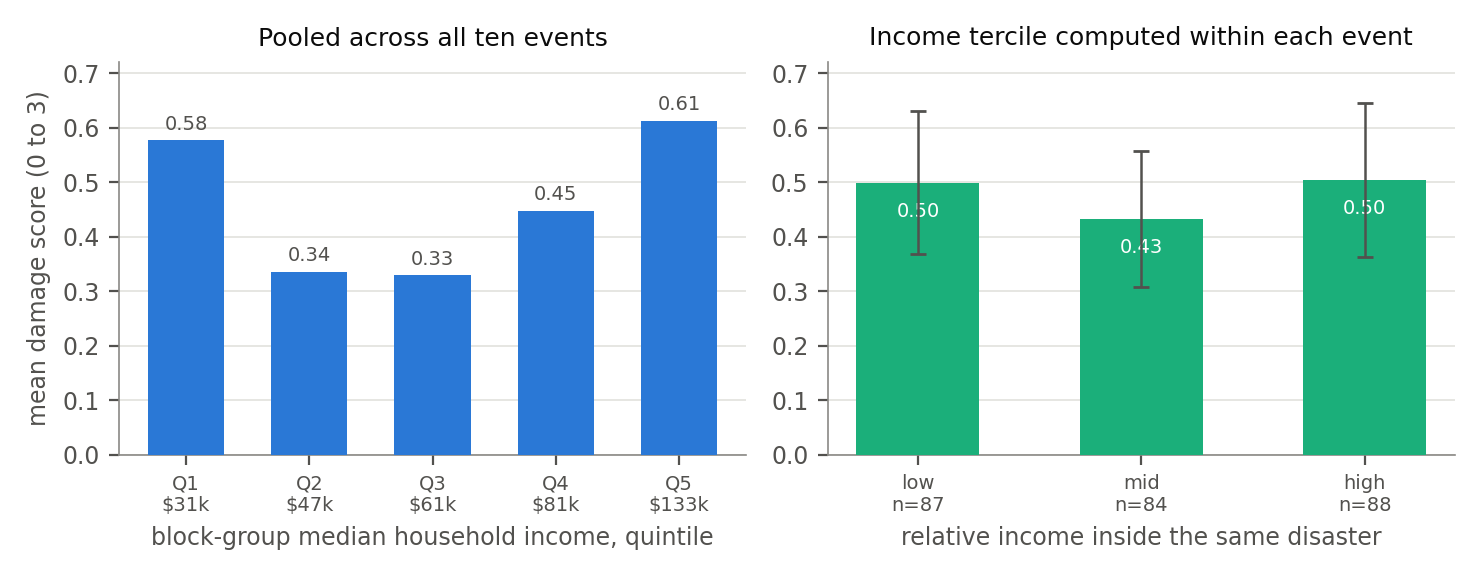
\includegraphics[width=0.85\textwidth]{figures/socio_income_gradient.png}
\caption{Left: pooling all ten events, mean damage score is U-shaped in income, highest in the
poorest and the richest quintiles and lowest in the middle. Right: once income terciles are computed
\emph{within} each event, the gradient flattens and the 95\% intervals overlap completely.}
\label{fig:socioincome}
\end{figure*}

Figure~\ref{fig:socioincome} shows the same thing without a model. Pooled across events the
relationship is U-shaped, not monotone: mean damage score is 0.58 in the poorest income quintile,
falls to 0.33 in the middle, and rises to 0.61 in the richest. That is what a mixture of two exposure
stories looks like, low-income tracts in tornado paths and high-income tracts in coastal and
wildland-urban-interface zones, rather than a single inequality gradient. Computing income terciles
\emph{within} each event, over the six events with at least 15 block groups, flattens it to
0.50 / 0.43 / 0.50, and the per-event direction is inconsistent in sign: damage rises with income
across \texttt{hurricane-\allowbreak harvey} (0.77 to 1.01) and falls with it across \texttt{joplin-tornado}
(0.90 to 0.41).

\begin{figure}[t]
\centering
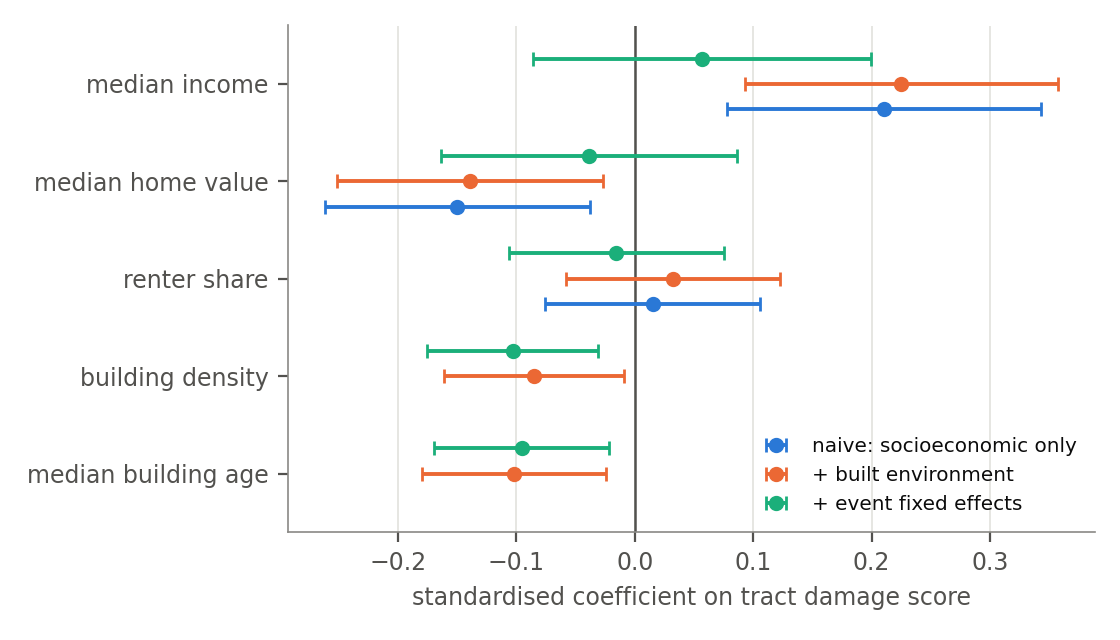
\includegraphics[width=\columnwidth]{figures/socio_coefficients.png}
\caption{Standardised coefficients with 95\% intervals across the three specifications. The two
socioeconomic effects shrink toward zero when event fixed effects enter; the two built-environment
effects do not.}
\label{fig:socioforest}
\end{figure}

What survives event fixed effects is the built environment: building density
($-0.103$, $p = 0.006$) and median building age ($-0.096$, $p = 0.012$) both remain significant and
barely move (Fig.~\ref{fig:socioforest}). Denser and older block groups record \emph{less} damage on
average, which runs against the usual intuition that older housing is more vulnerable, and is most
plausibly a settlement-pattern effect: dense, older cores sit away from the coastal and interface
edges where these particular hazards concentrate.

\subsection{What this means for deployment}

Two cautions follow, pointing the same way. First, the naive analysis would have supported a
confident and wrong policy claim: a pipeline that joined damage to income and reported the
coefficient would have published a significant positive income effect that does not survive the most
basic exposure control available, and the confounder is not subtle, it is simply which disaster hit
which place.

Second, this analysis runs on xBD \emph{ground-truth} labels, not model predictions, and that is
deliberate. Section~\ref{sec:results} showed the model's errors are not random: it over-flags
intermediate damage at a rate that depends on the disaster type. If error rates also correlate with
building density or housing type, and both correlate with income, running the same regression on
predicted damage would manufacture a socioeconomic finding out of model bias. Rapid automated damage
maps are genuinely useful for triage; using them as evidence for aid allocation, without verified
labels, risks encoding the model's calibration error as a claim about people.

% =====================================================================
\section{Limitations}

\begin{itemize}[leftmargin=*,itemsep=2pt,topsep=3pt]
\item \textbf{Thin out-of-domain support.} \class{minor} and \class{major} rest on 116 and 138 true
examples in \texttt{test\_ood}. These two classes drive the macro-F1 story, so their per-class figures
carry wide uncertainty.
\item \textbf{Annotator selection.} Every number is measured on buildings annotators were \emph{able}
to assess, since \class{un-classified} polygons are excluded, so true zero-shot difficulty is
somewhat higher than reported.
\item \textbf{Confounded geometry and partial checks.} The sun-elevation shift is inseparable from
event identity with only 19 events, the duplicate test covers 400 of 11,034 scenes, and model results
use a stratified sample of 1,698 scenes.
\item \textbf{Not a pure pretraining ablation}, since the encoders differ in initialisation and in
size (11.57M against 1.37M parameters); and model selection uses \texttt{val}, which is
in-distribution, because selecting on the out-of-domain set would leak the test set.
\item \textbf{Ecological inference in Part 3.} Block-group averages cannot support claims about
individual households, no true hazard-exposure layer was available, and ten events is a small basis
for fixed effects.
\end{itemize}

% =====================================================================
\section{Conclusions and next steps}

A siamese change-detection CNN trained on 14 non-fire disasters and evaluated zero-shot on five
wildfire events loses a third of its macro-F1, but the loss sits entirely in the two classes that
barely exist under wildfire, while destroyed-versus-intact discrimination \emph{improves}. ImageNet
pretraining helps on every split and every metric, and helps most out of domain. On the impact side,
damage here is not distributed along an income gradient once the disaster itself is controlled for.
Outstanding work, in priority order:

\begin{enumerate}[leftmargin=*,itemsep=2pt,topsep=3pt]
\item \textbf{Test the calibration hypothesis directly.} Apply prior correction~\cite{saerens} to the
out-of-domain predictions of both models and measure how much of the macro-F1 gap closes without
retraining. If most of it closes, that is the strongest result the project can report.
\item \textbf{Few-shot ablation}: add 1 to 5\% of wildfire scenes to training and re-measure the gap.
\item \textbf{Randomly initialised ResNet-18} as a third run, to separate pretraining from capacity.
\item \textbf{Real hazard-exposure layers} for Part 3, and a rerun of the same regression on
predicted rather than true damage, to quantify how much model bias would leak into the social
conclusion.
\end{enumerate}

\paragraph{Reproducibility.} \texttt{notebooks/\allowbreak 01\_eda.ipynb} and
\texttt{notebooks/\allowbreak 02\_data\_split.\allowbreak ipynb} run the full-dataset exploratory analysis, the cleaning
ledger and the event-stratified scene sampling locally without a GPU, writing to
\texttt{results/\allowbreak 01\_eda/} and \texttt{results/\allowbreak 02\_data\_split/}. Each model has its own training
notebook (\texttt{pretrained\_\allowbreak resnet18\_\allowbreak train.ipynb}, \texttt{train\_\allowbreak scratch\_\allowbreak cnn.ipynb}) reading the
same patch arrays, and \texttt{socio\_\allowbreak analysis.ipynb} covers Part 3. Every figure and table here is
generated from the CSV artefacts those notebooks write. Seed 42 throughout.

\paragraph{Contributions.} Artur Zavistovskyi: exploratory analysis, data cleaning and quality
diagnostics, patch pipeline, pretrained model, evaluation, this report. Bhuvanesh Dinesh Wadhwani:
dataset indexing and the train/val/test split design used here. Yitian Zhou: pretrained model
(joint). Anastasiia Khitrova: from-scratch CNN baseline and the impact analysis of
Section~\ref{sec:socio}.

% =====================================================================
\begin{thebibliography}{9}
\small

\bibitem{xbd}
R.~Gupta \emph{et al.},
``xBD: A Dataset for Assessing Building Damage from Satellite Imagery,''
\emph{arXiv:1911.09296}, 2019.

\bibitem{fusion}
E.~Weber and H.~Kan\'e,
``Building Disaster Damage Assessment in Satellite Imagery with Multi-Temporal Fusion,''
\emph{arXiv:2004.05525}, 2020.

\bibitem{resnet}
K.~He, X.~Zhang, S.~Ren and J.~Sun,
``Deep Residual Learning for Image Recognition,'' \emph{CVPR}, 2016.

\bibitem{imagenet}
J.~Deng \emph{et al.},
``ImageNet: A Large-Scale Hierarchical Image Database,'' \emph{CVPR}, 2009.

\bibitem{lpft}
A.~Kumar, A.~Raghunathan, R.~Jones, T.~Ma and P.~Liang,
``Fine-Tuning can Distort Pretrained Features and Underperform Out-of-Distribution,''
\emph{ICLR}, 2022.

\bibitem{saerens}
M.~Saerens, P.~Latinne and C.~Decaestecker,
``Adjusting the Outputs of a Classifier to New a Priori Probabilities,''
\emph{Neural Computation}, 14(1):21-41, 2002.

\bibitem{pytorch}
A.~Paszke \emph{et al.},
``PyTorch: An Imperative Style, High-Performance Deep Learning Library,'' \emph{NeurIPS}, 2019.

\bibitem{acs}
U.S. Census Bureau, American Community Survey 5-Year Estimates (2017) and TIGER/Line block-group
boundaries (2020).

\bibitem{xview2}
xView2 Challenge, \url{https://xview2.org}.

\end{thebibliography}

\end{document}
